%!TEX root = ../../msc17-game-book.tex


\phWorksheet{Solution - Bonus Puzzle 3}

The answer is \(7\) (of course, the proof that \(8\) is impossible is
non-trivial). Here's one such embedding:

\begin{center}
  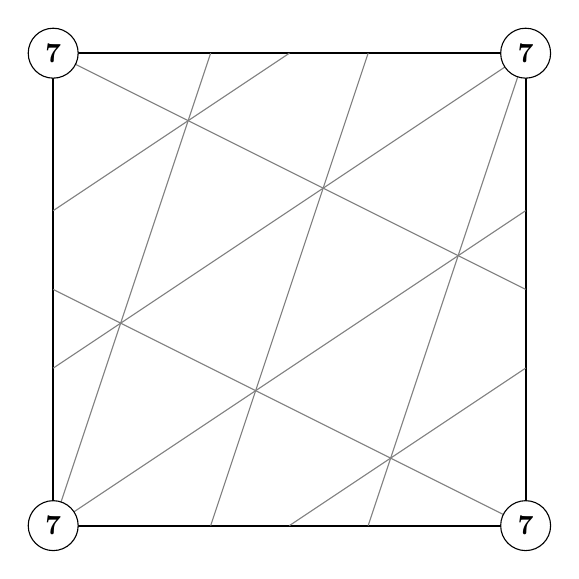
\begin{tikzpicture}
    \draw[thick] (0,0) rectangle (6,6);
    \draw[color=gray,thin] (0,0) -- +(2,6);
    \draw[color=gray,thin] (2,0) -- +(2,6);
    \draw[color=gray,thin] (4,0) -- +(2,6);
    \draw[color=gray,thin] (0,6) -- +(6,-3);
    \draw[color=gray,thin] (0,3) -- +(6,-3);
    \draw[color=gray,thin] (0,0) -- +(6,4);
    \draw[color=gray,thin] (0,4) -- +(3,2);
    \draw[color=gray,thin] (3,0) -- +(3,2);
    \draw[color=gray,thin] (0,2) -- +(6,4);
    \node[draw,circle,fill=white] at (0,0) {\bf 7};
    \node[draw,circle,fill=white] at (6,0) {\bf 7};
    \node[draw,circle,fill=white] at (0,6) {\bf 7};
    \node[draw,circle,fill=white] at (6,6) {\bf 7};
  \end{tikzpicture}
\end{center}
